\documentclass[letterpaper, 12 pt, conference]{ieeeconf}

\overrideIEEEmargins
% See the \addtolength command later in the file to balance
% the column lengths on the last page of the document

\usepackage{amsmath}
\usepackage{graphicx}
\usepackage{soul}
\setuldepth{1}
\usepackage{booktabs}
\usepackage{multirow}

\usepackage[style=ieee]{biblatex}
\bibliography{biblio}

\usepackage[dvipsnames]{xcolor}
\usepackage{hyperref}
\hypersetup{
    colorlinks=true,
    citecolor=blue,
    linkcolor=blue,
    filecolor=magenta,      
    urlcolor=blue,
}
\newcommand{\todo}[1]{\textcolor{red}{#1}}
\newcommand{\tocheck}[1]{\textcolor{blue}{#1}}


% The following packages can be found on http:\\www.ctan.org
%\usepackage{graphics} % for pdf, bitmapped graphics files
%\usepackage{epsfig} % for postscript graphics files
%\usepackage{mathptmx} % assumes new font selection scheme installed
%\usepackage{times} % assumes new font selection scheme installed
%\usepackage{amsmath} % assumes amsmath package installed
%\usepackage{amssymb}  % assumes amsmath package installed

\title{
    {\LARGE \bf Category Robustness\\}
    {\Large If it looks like a duck...}
}

\author{
Xavier Morin Duchesne\\% <-this % stops a space
M. Sc. Computer Science\\
School of Computer Science, McGill University\\
Course: COMP762 -- ML \& NLP Methods for Software Engineering 
}


%\usepackage{comment}

\begin{document}



\maketitle
\thispagestyle{empty}
\pagestyle{empty}

%%%%%%%%%%%%%%%%%%%%%%%%%%%%%%%%%%%%%%%%%%%%%%%%%%%%%%%%%%%%%%%%%%%%%%%%%%%%%%%%
\begin{abstract}
When designing a tool dependent on human-defined categories, it is important to keep in mind that such categories are inherently vague and their boundaries ambiguous. We propose a novel measure, category robustness, which can be used to evaluate the semantic boundaries between categories. We demonstrate that this novel measure is correlated with logical proxies for semantic closeness and demonstrate a possible use case for this novel measure.
\end{abstract}

%%%%%%%%%%%%%%%%%%%%%%%%%%%%%%%%%%%%%%%%%%%%%%%%%%%%%%%%%%%%%%%%%%%%%%%%%%%%%%%%
\section{Introduction}

% Elephant, blind men; different papers getting at something different?
% How do we avoid falling into the trap of blindly splitting up the elephant?

% Other idea: if it walks like a duck, quacks like a duck, and ... it must be a duck.
% But... platypus?
\textit{If it looks like a duck, swims like a duck, and quacks like a duck, then it must be a duck!} But what about the platypus? It shares some of the most defining physical characteristics of a duck, yet it is not a duck. Where, then, does one draw the line? When is a duck a duck and a platypus, a platypus?

Absurd as this example may seem, it highlights the inherent vagueness of categories. As Andersen put it ``semantic domains or `fields', as well as specific items within them, in a given language often seem to defy any kind of adequate, unique, unambiguous description.'' \cite{andersen:cups_and_glasses:1975} That is to say that, contrary to our intuition, categories are often vague and their boundaries fuzzy \cite{lehrer1970indeterminacy}. This vagueness and the lack of explicit semantic boundaries can in fact be shown to extend even to simple, common, everyday objects. Labov \cite{labov:boundares:1973}, for example, showed in his seminal work that the boundaries between common kitchenware such as cups, bowls, and vases, are fuzzy: Which physical features define a cup as a cup? More importantly, which physical features distinguish it from a bowl or vase? One could argue that the presence of a handle is defining of a cup, but a cup with a broken handle is still a cup. Similarly, size is an important yet insufficient factor: large cups and small bowls do exist.

These considerations---the inherent vagueness of real-world categories and the fuzziness of their semantic boundaries---are important to keep in mind when creating tools which depend on a set of human-defined categories. There are many instances in the Software Engineering literature \cite{disorbo:deca:2016, guzzi:developer_communication:2012, guzzi:communication_in_mailing_lists:2013, huang:aim:2018,  DiSorbo:app_reviews:2016, gu:app_reviews:2015, maalej:bug_feature_praise:2015, palomba:app_reviews:2017, panichella:app_reviews:2015, villarroel:app_reviews:2016, pagano:user_feedback:2013} where a set of categories was first induced through manual inspection of a sample of a larger dataset, and where, then, a method was devised to assign new content to these categories, having been designed to reproduce the human intuition which engendered the categories in the first place.  As argued earlier, however, human-defined categories, even those of simple, common, everyday objects, are inherently vague and lack well-defined semantic boundaries. This thus calls into question the quality of the categories proposed for such abstract concepts as developer communications \cite{disorbo:deca:2016, guzzi:developer_communication:2012, guzzi:communication_in_mailing_lists:2013, huang:aim:2018}, app reviews \cite{DiSorbo:app_reviews:2016, gu:app_reviews:2015, maalej:bug_feature_praise:2015, palomba:app_reviews:2017, panichella:app_reviews:2015, villarroel:app_reviews:2016}, or user feedback \cite{pagano:user_feedback:2013}, and the validity of the related methods. Importantly, this also highlights the need for tools for evaluating the vagueness of those semantic categories and their boundaries.

Accordingly, the goal of this project was to evaluate a novel measure, category robustness, the purpose of which is to assess the semantic boundaries between categories. The idea behind category robustness is that it should be possible to exchange components of members belonging to semantically close categories without affecting category membership.  To put it differently, exchanging parts between two cars yields two cars.\footnote{The resulting vehicles may not be functional or aesthetically pleasing, but we argue that they would no less be recognizable as cars.} Likewise, exchanging parts between a car and a plane, though likely to yield two useless piles of scrap metal, may yield a (strange looking) car and plane. Conversely, exchanging parts between a car and a human being or, say, between a beaver and a duck, can only lead to some strange monstrosity, or, in the case of the beaver and duck, platypuses. By that logic, then, for a given pair of categories, category robustness is evaluated by exchanging components in members of the respective categories and evaluating the number the number of ``platypuses'' thereby created, in contrast to the number of new elements created which, despite the exchange, continue to fall neatly within one category or the other.

In what follows, we report our evaluation of category robustness on the set of intention mining categories proposed by Huang et al. \cite{huang:aim:2018}. More specifically, we created augmented sentences by exchanging noun phrases within the sentences in the Huang et al. dataset, and evaluate how often these resulting augmented sentences fall within either of their original categories and how often platypuses are created. These measures are correlated to measures other measures of category similarity described below and insights about the relationships between categories are discussed.

Please note that although we focus, here, on intention mining and, specifically, on the work done by Huang et al. \cite{huang:aim:2018}, this approach is not specific to their dataset, nor is it specific to intention mining, and should be applicable to all areas of Software Engineering where categories have been proposed along with automated methods for assigning future content to those categories. 

\section{Related works}
\begin{figure}
    \centering
    \includegraphics[scale=0.8]{LabovFig5-mod.png}
    \caption{Objects 1--4 from \cite{labov:boundares:1973}, Figure~5, page~354. In his seminal work, Labov investigated the impact of variations on width, depth, and shape on our judgement of whether a given object is a cup or bowl. Only variations on width are shown here.}
    \label{fig:labov}
\end{figure}
In his seminal work, Labov \cite{labov:boundares:1973} investigated ambiguity in the ``denotation of cups and cuplike containers, and the use of words such as \ul{cup}, \ul{bowl}, \ul{dish}, \ul{mug}, \ul{glass}, \ul{pitcher}, etc. and their corresponding terms in other languages.''\footnote{Text was underlined in the original work; the format was copied here for the sake of exactitude.} He found that, when asked to name containers of various shapes, widths, and depths, human observers gradually (rather than sharply) shifted their identifications from cup to bowl or to vase (see Figure~\ref{fig:labov} for examples of the containers used by Labov). In other words, human observers displayed fuzzy boundaries which resulted in gradual, rather than sharp, changes in describing cuplike containers. Labov ultimately concluded that function appeared to be the most important factor in determining the label assigned to cuplike containers: a vase is a vase, because it can contain flowers.

Andersen \cite{andersen:cups_and_glasses:1975} followed up on this work by showing that young children first rely on physical features in order to name objects and that, in doing so, they tend to overextend words like ``cup'' to containers which an adult would name otherwise. As they age, however, they begin to rely less on perceptual properties and more strongly on functional properties, recognizing that categories are inherently vague and that, as stated above, a vase is a vase not necessarily by its inherent properties, but by the way that it is used. It is unclear however whether this recognition of the vagueness of categories and the fuzziness of semantic boundaries is domain-specific or generalizes to all categories.

Huang et al. \cite{huang:aim:2018} proposed a set of seven intention categories---aspect evaluation, feature request, information giving, information seeking, problem discovery, solution proposal, and meaningless\footnote{This category is mostly composed of messages thanking the developers for their work.}---and trained a Convolutional Neural Network (CNN) to classify sentences into those categories. The purpose of their work was to classify sentences in developer discussions in order to facilitate dissemination of the relevant information to the relevant people: bug reports to maintainers, feature requests to developers, praise to management, and so on. Their work was meant to improve upon the Di Sorbo et al. \cite{disorbo:deca:2016} set of six categories and corresponding linguistic patterns for assigning sentences to the categories. The Di Sorbo et al. work, in turn, was designed as an improvement over Guzzi et al. \cite{guzzi:communication_in_mailing_lists:2013}. In all three cases, it should be noted, the categories were produced following manual inspection of the data. That is to say that the categories were not defined according to strict criteria, but, instead, according to human intuition which, as argued previously, is likely to produce vague categories with fuzzy boundaries. We use the freely available Huang et al. dataset for the purposes of this project.

Previous Natural Language Processing work interested in producing augmented sentences has occurred in other areas such as Grammatical Error Correction \cite{kiyono:grammar:2019}. As far as we are aware, however, this work is the first to apply this kind of augmentation to the field of Software Engineering and more specifically to the analysis of boundaries between categories.

\section{Methodology}
\subsection{Dataset}
For the purposes of this project, we chose to use the data collected by by Huang et al. \cite{huang:aim:2018}. It comprised $6,400$ sentences: the $983$ sentences collected by Di Sorbo et al. \cite{disorbo:deca:2016} and $5,417$ developer discussion sentences collected over four projects: Bootstrap \cite{bootstrap}, Docker \cite{docker}, Tensorflow \cite{tensorflow}, and VSCode \cite{vscode}. Huang et al. assigned each of these sentences to one of seven categories: aspect evaluation, feature request, information giving, information seeking, problem discovery, solution proposal, and meaningless. The dataset were split into a training set ($90\%$ of the data) and a validation set ($10\%$).

\subsection{Text preprocessing}
Sentences were preprocessed using the Stanford Core NLP toolkit \cite{StanfordCoreNLP}; punctuation and stop words were removed, and the remaining words were lemmatized. Words were marked with a part-of-speech tag and with a tag corresponding to their most immediate phrase (e.g., noun phrases).

\subsection{Machine learning models and analyses}
Analyses and machine learning models were written in Python 3 \cite{python3}, and ran on Google Colaboratory \cite{Colab}. They relied mainly on three Python libraries: Numpy \cite{numpy}, Scikit-learn \cite{scikit-learn}, and PyTorch \cite{pytorch}. 

Three machine learning models were used to evaluate category robustness: Support Vector Machines \cite{chang:libsvm:2011}, a Long Short-Term Memory model \cite{hochreiter:lstm:1997}, and the Huang et al. Convolutional Neural Network \cite{huang:aim:2018}.

For the SVM model, a processing pipeline was created where sentences were first transformed to a bag-of-words representation, before being to a TF-IDF representation \cite{baeza:tfidf:1999}. The TFIDF vectors corresponding to each sentence where finally fed to the Support Vector classifier which used a linear kernel with $C = 1$.

For the LSTM, words were passed through an embedding layer of size 128 before being passed to the LSTM itself. The LSTM had two layers with 256 hidden states each.

Finally, similarly to the LSTM, words first passed through an embedding layer of size 128 before being passed to the CNN itself. The CNN was composed of three parallel convolutional layers with filter sizes of 3, 4, and 5 respectively. The output of these layers was given to a dropout layer, followed by a rectified linear unit, before being concatenated and finally given to a linear classifier. See \cite{huang:aim:2018} for more details.

\subsection{Term-based methods}
Two term-based methods were used: TF-IDF \cite{baeza:tfidf:1999} and In-Out scores.

TF-IDF or term frequency-inverse document frequency is a measure commonly used to identify important terms within a set of documents. It gives high scores to terms which occur frequently in few documents and low scores to terms which occur frequently across documents. This is meant, for example, to give low scores to common words such as the article ``the'' or the verb ``to be.''

The In-Out score was created specifically for our purposes and it is defined as follows:\\[2em]
$\mathrm{In}-\mathrm{Out_{W, C}} =$
\begin{align*}\hspace{-.30cm}
z \left(\# \textrm{occurrences of } W \textrm{ in } C\right)
\end{align*}\vspace{-1cm}
\begin{align*}
- z \left(\# \textrm{occurrences of } W \textrm{ not in } C\right)
\end{align*}

where $z()$ calculates the z-score, and $W$ and $C$ are respectively the word and category of interest. Using this measure, we obtain a score for each word and category representing the importance of that word to that category.

\begin{figure}
    \centering
    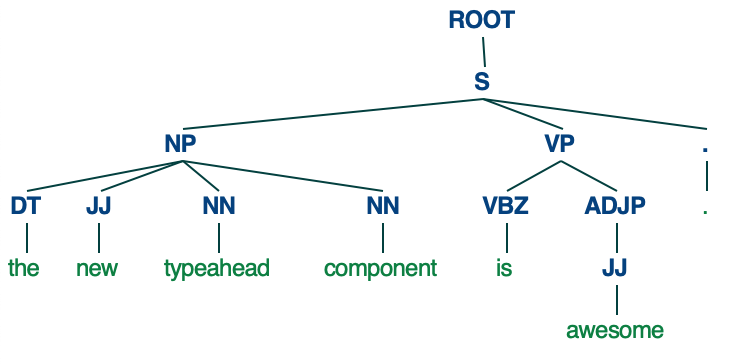
\includegraphics[scale=.68]{parse_tree.png}
    \caption{Example of a parse tree.}
    \label{fig:parse_tree}
\end{figure}
\begin{table}[tp]
    \centering
    \begin{tabular}{lcccccccc}
        \toprule
            & &
            \multicolumn{1}{c}{\textbf{AE}} & \multicolumn{1}{c}{\textbf{FR}} & \multicolumn{1}{c}{\textbf{IG}} & \multicolumn{1}{c}{\textbf{IS}} & \multicolumn{1}{c}{\textbf{PD}} & \multicolumn{1}{c}{\textbf{SP}} & \multicolumn{1}{c}{\textbf{ML}} \\
        \midrule
        \multirow{2}{*}{\textbf{TF-IDF}} & \textit{POS} & N & N & N & N & N & N & N \\
        & \textit{phrase} & NP & NP & NP & NP & NP & NP & NP \\
        \midrule
        \multirow{2}{*}{\textbf{In-Out}} & \textit{POS} & J & J & N & N & N & N & J \\
        & \textit{phrase} & JP & JP & NP & NP & NP & NP & NP \\
        \bottomrule
    \end{tabular}
    \caption{The parts of speech and phrases which presented the highest total TFIDF score and highest total In-Out score for each category.\\N = noun, J = adjective, NP = noun phrase, JP = adjective phrase}
    \label{table:most-important}
\end{table}

\subsection{Sentence augmentation}
For the purposes of this report, augmented sentences were created using a new method: phrase swapping. In phrase swapping, phrases (e.g., noun phrases) in two different sentences are identified and swapped. For example, let us consider the following pair of sentences:\\[0.35em]
\indent{}\ul{The new typeahead component} is awesome.\\
\indent{}We need \ul{a dark/inverted style alert} for this.\\[0.45em]
\noindent{}where the first sentence is part of the ``aspect evaluation'' category and the second, ``feature request.'' In each of these sentences, a noun phrase has been identified and underlined. We can swap these noun phrases across sentences to obtain:\\[0.35em]
\indent{}\ul{A dark/inverted style alert} is awesome.\\
\indent{}We need \ul{the new typeahead component} for this.\\[1em]
\indent{}Programmatically, this is achieved using the Stanford Core NLP toolkit \cite{StanfordCoreNLP}. The toolkit is used to obtain a parse tree for each sentence (see Figure~\ref{fig:parse_tree} for an example); it is then simply a question of identifying subtrees in each sentence with the appropriate chunk type and swapping them. 

\begin{table}[tbp]
    \centering
    \begin{tabular}{lccccccc}
        \toprule
            &
            \multicolumn{1}{c}{\textbf{AE}} & \multicolumn{1}{c}{\textbf{FR}} & \multicolumn{1}{c}{\textbf{IG}} & \multicolumn{1}{c}{\textbf{IS}} & \multicolumn{1}{c}{\textbf{PD}} & \multicolumn{1}{c}{\textbf{SP}} & \multicolumn{1}{c}{\textbf{ML}} \\
        \midrule
            \textbf{AE} & & .90 & .91 & .65 & .73 & .70 & .60 \\
            \textbf{FR} & &     & .83 & .55 & .61 & .59 & .52 \\
            \textbf{IG} & &     &     & .87 & .88 & .83 & .80 \\
            \textbf{IS} & &     &     &     & .62 & .55 & .45 \\ 
            \textbf{PD} & &     &     &     &     & .66 & .50 \\ 
            \textbf{SP} & &     &     &     &     &     & .47 \\ 
            \textbf{ML} & &     &     &     &     &     &     \\ 
        \bottomrule
    \end{tabular}
    \caption{Category robustness scores for each pair of categories as calculated by the SVM.}
    \label{table:svm}
\end{table}
\begin{table}[t!]
    \centering
    \begin{tabular}{lccccccc}
        \toprule
            &
            \multicolumn{1}{c}{\textbf{AE}} & \multicolumn{1}{c}{\textbf{FR}} & \multicolumn{1}{c}{\textbf{IG}} & \multicolumn{1}{c}{\textbf{IS}} & \multicolumn{1}{c}{\textbf{PD}} & \multicolumn{1}{c}{\textbf{SP}} & \multicolumn{1}{c}{\textbf{ML}} \\
        \midrule
            \textbf{AE} & & .92 & .89 & .92 & .86 & .83 & .88 \\
            \textbf{FR} & &     & .83 & .86 & .76 & .75 & .82 \\
            \textbf{IG} & &     &     & .91 & .89 & .81 & .85 \\
            \textbf{IS} & &     &     &     & .88 & .82 & .86 \\ 
            \textbf{PD} & &     &     &     &     & .82 & .86 \\ 
            \textbf{SP} & &     &     &     &     &     & .80 \\ 
            \textbf{ML} & &     &     &     &     &     &     \\ 
        \bottomrule
    \end{tabular}
    \caption{Category robustness scores for each pair of categories as calculated by the LSTM.}
    \label{table:lstm}
\end{table}
\begin{table}[t!]
    \centering
    \begin{tabular}{lccccccc}
        \toprule
            &
            \multicolumn{1}{c}{\textbf{AE}} & \multicolumn{1}{c}{\textbf{FR}} & \multicolumn{1}{c}{\textbf{IG}} & \multicolumn{1}{c}{\textbf{IS}} & \multicolumn{1}{c}{\textbf{PD}} & \multicolumn{1}{c}{\textbf{SP}} & \multicolumn{1}{c}{\textbf{ML}} \\
        \midrule
            \textbf{AE} & & .89 & .94 & .94 & .85 & .80 & .86 \\
            \textbf{FR} & &     & .98 & .83 & .72 & .72 & .79 \\
            \textbf{IG} & &     &     & .94 & .93 & .86 & .87 \\
            \textbf{IS} & &     &     &     & .84 & .80 & .81 \\ 
            \textbf{PD} & &     &     &     &     & .79 & .79 \\ 
            \textbf{SP} & &     &     &     &     &     & .91 \\ 
            \textbf{ML} & &     &     &     &     &     &     \\ 
        \bottomrule
    \end{tabular}
    \caption{Category robustness scores for each pair of categories as calculated by the Huang et al. CNN \cite{huang:aim:2018}}
    \label{table:cnn}
\end{table}

\section{Results and Discussion}
One of the pitfalls of exploratory studies like this one is that there are often a large number of directions that the study can take with little-to-no guidance on which direction it should take. In our case, for example, swapping noun phrases seemed like an obvious choice, but swapping verb phrases and substituting verbs also seemed interesting. Unfortunately, swapping verb phrases is more complex: one verb may be transitive and the other intransitive; one verb may be conjugated for a third person pronoun (e.g., he has) whereas the other is conjugated for a first pronoun (I find). It was thus important for us to investigate further before investing time and effort into creating heuristics which may turn out not to be useful.
\begin{table}[tp!]
    \centering
    \begin{tabular}{lccccccc}
        \toprule
            &
            \multicolumn{1}{c}{\textbf{AE}} & \multicolumn{1}{c}{\textbf{FR}} & \multicolumn{1}{c}{\textbf{IG}} & \multicolumn{1}{c}{\textbf{IS}} & \multicolumn{1}{c}{\textbf{PD}} & \multicolumn{1}{c}{\textbf{SP}} & \multicolumn{1}{c}{\textbf{ML}} \\
        \midrule
            \textbf{AE} & & .53 & .50 & .47 & .35 & .40 & .24 \\
            \textbf{FR} & &     & .53 & .50 & .43 & .44 & .20 \\
            \textbf{IG} & &     &     & .55 & .47 & .53 & .19 \\
            \textbf{IS} & &     &     &     & .45 & .47 & .26 \\ 
            \textbf{PD} & &     &     &     &     & .50 & .17 \\ 
            \textbf{SP} & &     &     &     &     &     & .19 \\ 
            \textbf{ML} & &     &     &     &     &     &     \\ 
        \bottomrule
    \end{tabular}
    \caption{Proportion of overlap between pairs of categories in the top-100 words with the highest TF-IDF scores.}
    \label{table:over-tfidf}
\end{table}

\begin{table}[tp!]
    \centering
    \begin{tabular}{lccccccc}
        \toprule
            &
            \multicolumn{1}{c}{\textbf{AE}} & \multicolumn{1}{c}{\textbf{FR}} & \multicolumn{1}{c}{\textbf{IG}} & \multicolumn{1}{c}{\textbf{IS}} & \multicolumn{1}{c}{\textbf{PD}} & \multicolumn{1}{c}{\textbf{SP}} & \multicolumn{1}{c}{\textbf{ML}} \\
        \midrule
            \textbf{AE} & & .08 & .03 & .03 & .00 & .02 & .09 \\
            \textbf{FR} & &     & .05 & .04 & .02 & .04 & .06 \\
            \textbf{IG} & &     &     & .17 & .05 & .09 & .01 \\
            \textbf{IS} & &     &     &     & .04 & .10 & .06 \\ 
            \textbf{PD} & &     &     &     &     & .05 & .00 \\ 
            \textbf{SP} & &     &     &     &     &     & .00 \\ 
            \textbf{ML} & &     &     &     &     &     &     \\ 
        \bottomrule
    \end{tabular}
    \caption{Proportion of overlap between pairs of categories in the top-100 words with the highest In-Out scores.}
    \label{table:over-inout}
\end{table}
\begin{table}[tp!]
    \centering
    \begin{tabular}{lccccccc}
        \toprule
            &
            \multicolumn{1}{c}{\textbf{SVM}} & \multicolumn{1}{c}{\textbf{LSTM}} & \multicolumn{1}{c}{\textbf{CNN}} & \multicolumn{1}{c}{\textbf{TF-IDF}} & \multicolumn{1}{c}{\textbf{In-Out}} \\
        \midrule
            \textbf{SVM}    & & .60 & .40 & .60 & .28 \\
            \textbf{LSTM}   & &     & .85 & .36 & .32 \\
            \textbf{CNN}    & &     &     & .25 & .27 \\
            \textbf{TF-IDF} & &     &     &     & .44 \\ 
            \textbf{In-Out} & &     &     &     &     \\ 
        \bottomrule
    \end{tabular}
    \caption{Correlations between the different measures of category robustness and category overlap.}
    \label{table:correlations}
\end{table}


Our first step was therefore to use term-based methods, TF-IDF and In-Out scores, in order to identify the most important parts-of-speech and phrases in our dataset. In order to do so, each category's sentences into a single document and calculated a TF-IDF score for each word in those documents. We similarly calculated an In-Out score for word and category. We then calculated part-of-speech and phrase scores by summing the scores of words assigned with the part-of-speech or part of the phrase type. The results, presented in Table~\ref{table:most-important}, suggest that nouns and noun phrases were the most important part-of-speech and phrase, respectively. We accordingly focus on noun phrases in what follows.

Our second step was to create augmented sentences by swapping noun-phrases between sentences of the same and different categories, and to use the three models, SVM, LSTM, and CNN, trained beforehand on the Huang et al. \cite{huang:aim:2018} data, to assign categories to the new augmented sentences. As discussed earlier, the idea is that exchanges between semantically close categories are more likely to produce augmented sentences which still fit in those categories (i.e., a duck or a beaver), whereas exchanges between semantically far categories (robust categories) are more likely to create sentences which fit in neither (i.e., platypuses). The results are displayed in Tables~\ref{table:svm}, \ref{table:lstm}, and \ref{table:cnn} for the SVM, LSTM, and CNN respectively.


Having now evaluated category robustness using three machine learning models, we wanted to confirm that category robustness was actually getting at something, some inherent properties of those categories. In order to do so, we calculated overlap scores for each category pair using both TF-IDF and In-Out. That is to say that, for each category, we obtained the top 100 words with the highest TF-IDF and In-Out scores and then counted the number of words shared between pairs of categories. Both TF-IDF and In-Out scores are meant to represent the importance of words; if a given word is important to two categories, this suggests that those categories are closer than if that that word were not important to both. Therefore, by measuring this overlap, we can get an idea of the semantic distance between categories. The results are presented in Tables~\ref{table:over-tfidf}~and~\ref{table:over-inout}. Of note, the In-Out overlap scores are far lower than those for TF-IDF. This is not surprising: the In-Out measure was designed explicitly to identify words that are important to a category, but not to to others. Having obtained measures of word overlap, we compared all of the available measures to each other and display the results in Table~\ref{table:correlations}. Interestingly, all correlations are greater than zero and would qualify, at the very least, as small correlations (between $.2$ and $.3$), with some correlations which would even qualify as large ($.60$ and $0.85$). This suggests that category robustness does embody a property of categories related to the ambiguity of semantic boundaries.

Finally, it is worth mentioning that Multidimensional Scaling\cite{mds} can be applied to category robustness scores (for example those of the CNN, reported in Table~\ref{table:cnn}) in order to obtain a visualization of the relationship between categories (like the one in Figure~\ref{fig:mds}). In a such a graph, points that are close together represent categories that are semantically closer, whereas points that are far away represent categories that more mutually robust.

\begin{figure}
    \centering
    \includegraphics[scale=0.5]{MDS.png}
    \caption{The relationships between categories as ascertained by the Huang et al. \cite{huang:aim:2018} CNN, represented in two dimensions using Multidimensional Scaling. Categories that are close in this graph were found to be close semantically as well.}
    \label{fig:mds}
\end{figure}


\section{Conclusion}
Human-defined categories are inherently vague and their boundaries fuzzy. We set out to explore a novel measure, category robustness, for evaluating the boundaries between categories. We found that our measure correlates well with other, common-sense measures of similarity between categories. Finally, we combine our approach with Multidimensional Scaling to get insights into the relationships between categories.

% The following command serves to balance the column lengths
% on the last page of the document manually. It shortens
% the textheight of the last page by a suitable amount.
% This command does not take effect until the next page
% so it should come on the page before the last. Make
% sure that you do not shorten the textheight too much.
%\addtolength{\textheight}{-2.5cm} 
                                 
                                 
                                 
                                 
                                 


\printbibliography

\end{document}
